\chapter{Objetivos e características}

Os objetivos do gerenciamento do escopo do projeto são: definir o que está e o que não está incluso no projeto e assegurar que o projeto inclui todo o trabalho necessário, e \textbf{apenas o necessário}, para terminar o projeto com sucesso.

Os processos que fazem parte do gerenciamento do escopo, representados na Figura \ref{fig:proc:ger:escopo}, podem ser resumidos em:

\begin{description}
	
	\item[\textbf{Coletar os requisitos}]: definir e documentar as necessidades das partes interessadas para alcançar os objetivos do projeto.
	
	\item[\textbf{Definir o escopo}]: desenvolver uma descrição detalhada do projeto e do produto.
	
	\item[\textbf{Criar a EAP}]: subdividir as entregas e o trabalho do projeto em componentes menores e mais facilmente gerenciáveis.
	
	\item[\textbf{Verificar o escopo}]: formalizar a aceitação das entregas terminadas do projeto.
	
	\item[\textbf{Controlar o escopo}]: monitorar o progresso do escopo do projeto e escopo do produto e gerenciar as mudanças feitas na linha de base do escopo.	

\end{description}

\begin{figure}[!h]
	\centering
	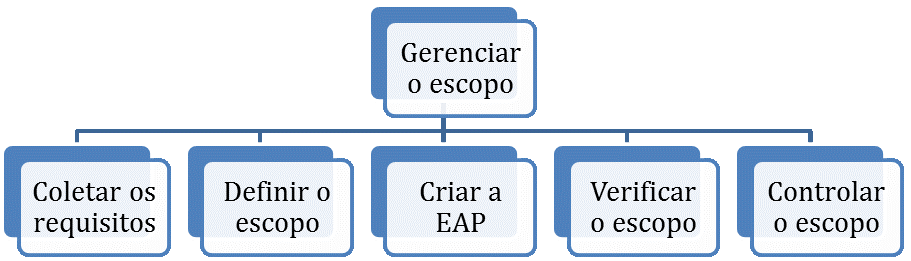
\includegraphics[scale=0.75]{Figuras/gerenciamento_escopo.png}
	\caption{Processos do Gerenciamento do escopo}
	\label{fig:proc:ger:escopo}
\end{figure}

Os processos dentro do ciclo de vida do projeto podem ser observados na Figura \ref{fig:ciclo:vida}.

\begin{figure}[!h]
	\centering
	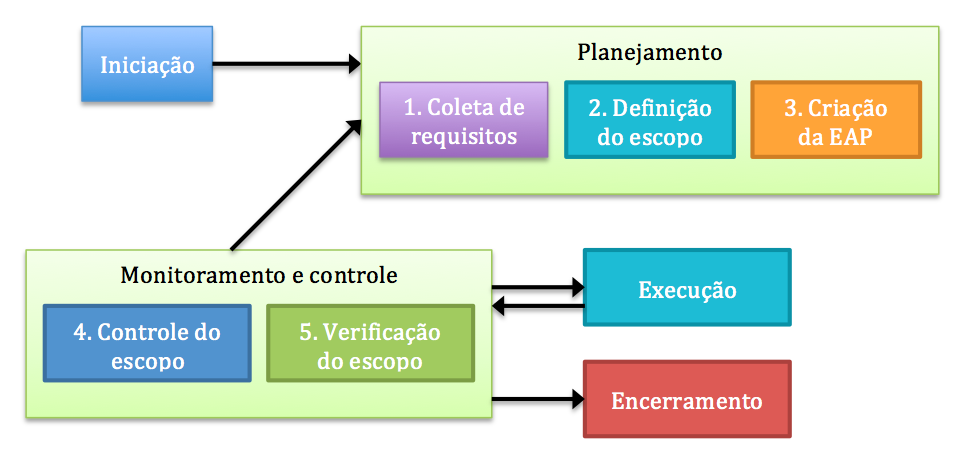
\includegraphics[scale=0.5]{Figuras/ciclo_vida.png}
	\caption{Processos dentro do ciclo de vida do projeto}
	\label{fig:ciclo:vida}
\end{figure}

\section{O que é escopo}

\begin{description}
	
	\item[Escopo do projeto:] os atributos e funções que caracterizam um produto, serviço ou resultado;
	
	\item[Escopo do projeto:] trabalho executado para entregar um produto, serviço ou resultado com os atributos e funções especificados.
	
\end{description}

O relacionamento entre o escopo do produto e do projeto pode ser observado na Figura \ref{fig:escopo:proj:prod}.

\begin{figure}[!h]
\centering
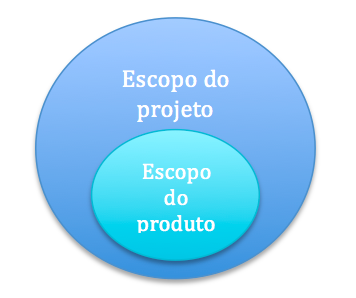
\includegraphics[scale=0.5]{Figuras/escopo_proj_prod.png}
\caption{Escopo produto X escopo projeto}
\label{fig:escopo:proj:prod}
\end{figure}

\section{Inimigos do escopo}

Um escopo com problemas pode levar o projeto ao seu fim. Por isso é importante observar os dois principais inimigos do escopo:

\begin{itemize}
	
	\item \textbf{\textit{Scope Creep}}: aumento do escopo sem nenhum controle, de maneira contínua, muitas vezes de forma lenta, que resulta em um escopo ``inchado'', ingerenciável, cujo foco foge da ideia inicial do projeto e o resultado reflete no aumento dos custos e perda de prazos.
	
	\item \textbf{\textit{Gold Plating}}: adicionar elementos não especificados nos requisitos do projeto, geralmente partindo de equipes técnicas e de desenvolvimento sob a alegação de agregar valor mas cujo resultado é o aumento de custos, perda de qualidade e aumento desnecessário da complexidade do produto.
	
\end{itemize}

\chapter{Planejar gerenciamento do escopo}

O plano de gerenciamento do escopo define como o escopo será definido, validado e controlado.

O processo de planejar o gerenciamento do escopo está representado na Figura \ref{fig:escopo:plan:efts} e será descrito a seguir.

\begin{figure}[!h]
	\centering
	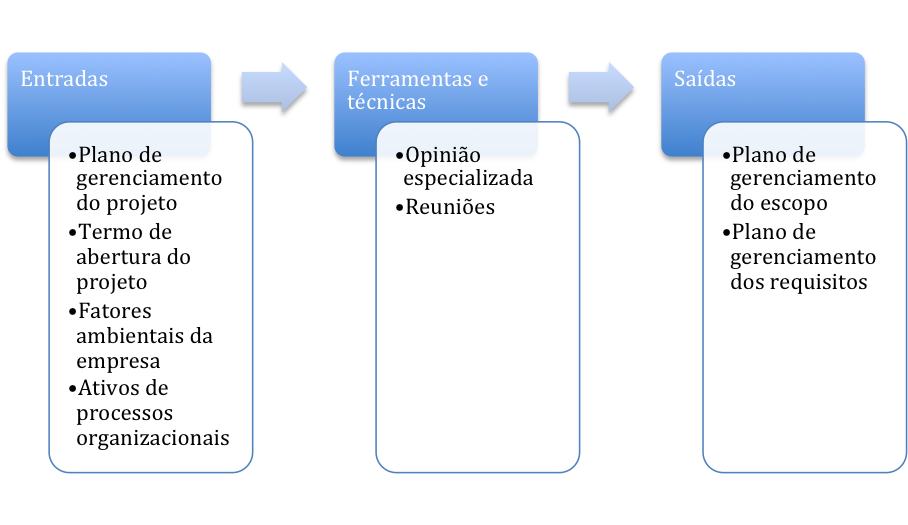
\includegraphics[scale=0.5]{Figuras/escopo_efts_planejar.png}
	\caption{Planejar o gerenciamento do escopo: entradas, ferramentas, técnicas e saídas}
	\label{fig:escopo:plan:efts}
\end{figure}

\section{Entradas}

\begin{description}
	
	\item[Plano de gerenciamento do projeto:] guia a forma de planejar e gerenciar o escopo.

	\item[Termo de abertura do projeto:] oferece o contexto necessário para planejar o gerenciamento do escopo, como descrição de alto nível e características do produto.

	\item[Fatores ambientais da empresa:] cultura, infraestrutura, etc.

	\item[Ativos de processos organizacionais:] políticas e procedimentos internos, informações históricas, lições aprendidas, etc.

\end{description}

\section{Ferramentas e técnicas}

\begin{description}

	\item[opinião especializada:] qualquer pessoa ou grupo que tenha conhecimento, habilidades, experiência ou treinamento em desenvolvimento do planejamento do escopo.

	\item[Reuniões:] podem participar o gerente de projetos, o patrocinador, membros selecionados da equipe, partes interessadas também selecionadas, entre outros.
	
\end{description}

\section{Saídas}

\begin{description}
	
	\item[Plano de gerenciamento do escopo:] é um componente do \planproj e descreve como o escopo será definido, desenvolvido, monitorado, controlado e verificado.

	\item[Plano de gerenciamento dos requisitos:] também é um componente do \planproj e define como os requisitos serão analisados, documentados e gerenciados.
	
\end{description}

\chapter{Coletar requisitos}

Processo de determinar, documentar e gerenciar necessidades das partes interessadas e requisitos para atingir os objetivos do projeto. 

Os requisitos podem ser classificados de várias formas. De acordo com o \bok, é comum se classificar os requisitos da seguinte forma:

\begin{description}
	
	\item[Requisitos de negócio:] necessidades de alto nível da organização, como ameaças e oportunidades.
	
	\item[Requisitos das partes interessadas:] necessidades das partes interessadas.
	
	\item[Requisitos da solução:] aspectos, funções e características dos produtos, serviços ou soluções do projeto. Podem ser ainda subdividos em dois grupos:
	
		\begin{description}
			
			\item[Funcionais:] descrevem o comportamento do produto.
			
			\item[Não funcionais:] complementam os requisitos funcionais e descrevem condições ambientais ou qualidades necessárias para que o produto seja efetivo.
			
		\end{description}
		
	\item[Requisitos de transição:] descevem capacidades temporárias, tais como conversões de dados ou treinamentos, necessários para a transição do estado atual para o estado desejado.
	
	\item[Requisito de projeto:] ações, processos ou outras condições que o projeto deva atender.
	
	\item[Requisitos de qualidade:] condições ou critérios necessários para validar a finalização com sucesso de uma entrega ou o cumprimento de outro requisito do projeto.
		
\end{description}
O processo de coletar requisitos está representado na Figura \ref{fig:escopo:req:efts} e será descrito a seguir.

\begin{figure}[!h]
	\centering
	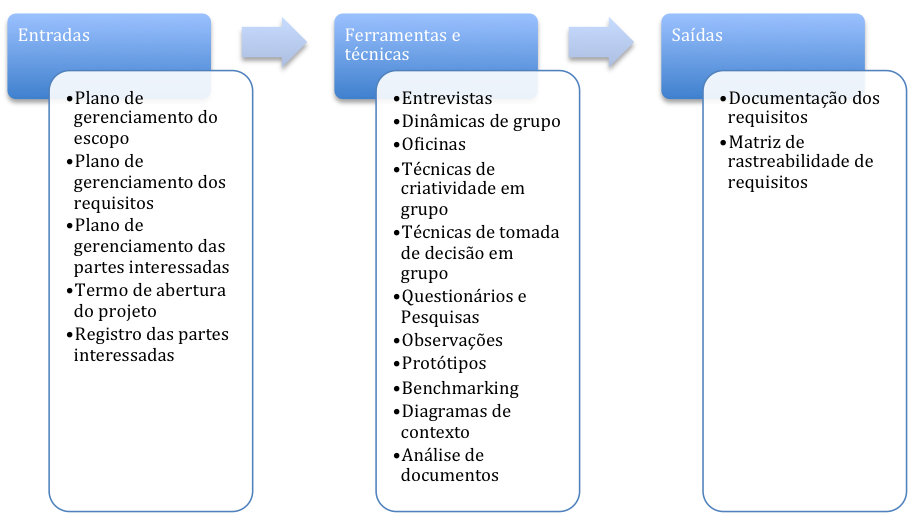
\includegraphics[scale=0.5]{Figuras/escopo_efts_requisitos.png}
	\caption{Coletar requisitos: entradas, ferramentas, técnicas e saídas}
	\label{fig:escopo:req:efts}
\end{figure}

\section{Entradas}

\begin{description}

	\item[Plano de gerenciamento do escopo:] esclarece como a equipe irá determinar quais requisitos necessitam de ser coletados.

	\item[Plano de gerenciamento dos requisitos:] oferece o processo que será usado para a coleta dos requisitos.

	\item[Plano de gerenciamento das partes interessadas:] usado para entender os requisitos de comunicação com as partes interessadas e o nível de engajamento deles avaliar e adaptar o seu nível de participação nas atividades de requisitos.

	\item[Termo de abertura do projeto:] oferece a descrição em alto nível dos produtos e serviços para que os requisitos possam ser detalhados.

	\item[Registro das partes interessadas:] usado para identificar as partes interessadas que podem prover informações sobre os requisitos e também como fonte das expectativas das partes interessadas e dos requisitos principais.

\end{description}

\section{Ferramentas e técnicas}

\begin{description}
	
	\item[Entrevistas:] formal ou informal, é a maneira de levantar as expectativas e requisitos diretamente com as partes interessadas.
	
	\item[Dinâmicas de grupo:] servem para juntar as partes interessadas e especialistas, também para levantar as expectativas e requisitos.
	
	\item[Oficinas:] mesma estratégia das dinâmicas de grupo, com grupos mais focados.
	
	\item[Técnicas de criatividade em grupo:] algumas técnicas podem ser utilizadas para facilitar o levantamento dos requisitos, tais como brainstorming, mapa mental, diagrama de afinidades, entre outros.
	
	\item[Técnicas de tomada de decisão em grupo:] técnicas de escolha entre diversas alternativas, podendo ser por unanimidade, majoritariedade, pluralidade ou ditatorial.
	
	\item[Questionários e Pesquisas:] servem para levantar informações de uma grande quatidade de pessoas rapidamente.
	
	\item[Observações:] particularmente útil para processos detalhados, é realizado através da observação de pessoas em seus ambientes executando trabalhos, tarefas ou processos.
	
	\item[Protótipos:] é uma forma de se obter respostas rapidamente através do fornecimento de modelos funcionais do produto esperado antes de sua construção final.
	
	\item[Benchmarking:] comparação das suas práticas (processos/operações) com as realizadas por outras organizações para servir de base de medição de performance.
	
	\item[Diagramas de contexto:] descrevem visualmente o escopo do produto exibindo um sistema de negócio e como as pessoas e outros sistemas interagem com ele.
	
	\item[Análise de documentos:] buscar e analisar documentos pré-existentes permite identificar informações relevantes para o levantamento de requisitos.
		
\end{description}

\section{Saídas}

\begin{description}
	
	\item[Documentação dos requisitos:] descreve como cada requisito contribui para alcançar os objetivos de negócio do projeto. Podem começar como requisitos de alto nível e serem masi detalhados conforme mais informações se obtém sobre os mesmos. Antes de serem colocados na linha de base, os requisitos devem ser:
	
		\begin{itemize}
			\item não ambíguos (mensuráveis e testáveis),
			\item rastreáveis,
			\item completos,
			\item consistentes e
			\item aceitáveis para pessoas interessadas chaves.
		\end{itemize}
	
	\item[Matriz de rastreabilidade de requisitos:] grade que liga os requisitos dos produtos desde sua origem até as entregas que os satisfazem.
	
\end{description}

\chapter{Definir o escopo}

Processo de desenvolver uma descrição detalhada do projeto e do produto. 

O processo de definir o escopo está representado na Figura \ref{fig:escopo:def:efts} e será descrito a seguir.

\begin{figure}[!h]
	\centering
	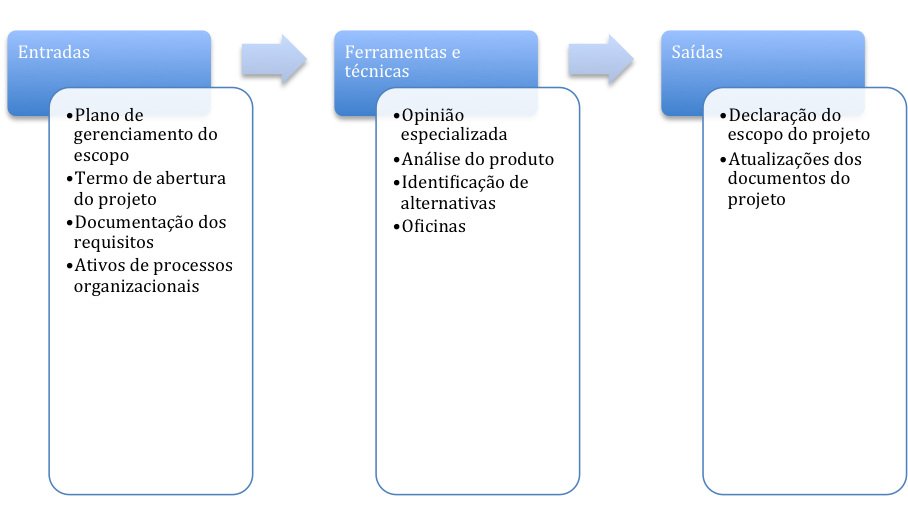
\includegraphics[scale=0.5]{Figuras/escopo_efts_definir.png}
	\caption{Definir o escopo: entradas, ferramentas, técnicas e saídas}
	\label{fig:escopo:def:efts}
\end{figure}

\section{Entradas}

\begin{description}
	
	\item[Plano de gerenciamento do escopo:] estabelece as atividades para desenvolver, monitorar e controlar o escopo do projeto.
	
	\item[Termo de abertura do projeto:] oferece a descrição em alto nível dos produtos e serviços.
	
	\item[Documentação dos requisitos:] será utilizado para selecionar os requisitos que serão incluídos no projeto
	
	\item[Ativos de processos organizacionais:] políticas, procedimentos, modelos, lições aprendidas, etc.
	
\end{description}

\section{Ferramentas e técnicas}

\begin{description}

	\item[Opinião especializada:] utilizada para analisar as informações necessárias para desenvolver o escopo.
	
	\item[Análise do produto:] diversos métodos, que variam conforme a área de atuação, podem ser utilizados para análise do produto, tais como análise de sistemas, análise de requisitos, engenharia de sistemas, engenharia de valores e análise de valores.
	
	\item[Geração de alternativas:] técnica utilizada para desenvolver tantas opções ponteciais quanto possíveis para identificar diferentes formas de se executar o trabalho do projeto.
	
	\item[Oficina:] servem para juntar as partes interessadas e especialistas a fim de atingir um acordo comum sobre os objetivos e limites do projeto.
	
\end{description}

\section{Saídas}

\begin{description}
	
	\item[Declaração do escopo do projeto:] descrição do escopo do projeto, principais entregas, premissas e restrições. Documenta completamente o escopo, incluindo o escopo do projeto e do produto. Descreve em detalhes as entregas e o trabalho necessário para criar essas entregas.
	
	\item[Atualizações dos documentos do projeto:] alguns documentos podem sofrer alterações no decorrer do desenvolvimento do escopo, tais como o registro de partes interessadas, a documentação de requisitos e a matriz de rastreabilidade dos requisitos.
	
\end{description}

\chapter{Criar a EAP}

Criar a Estrutura Analítica do Projeto (EAP) é o processo de subdividir as entregas e o trabalho do projeto em componentes menores e mais gerenciáveis.

O processo de criar a EAP está representado na Figura \ref{fig:escopo:eap:efts} e será descrito a seguir.

\begin{figure}[!h]
	\centering
	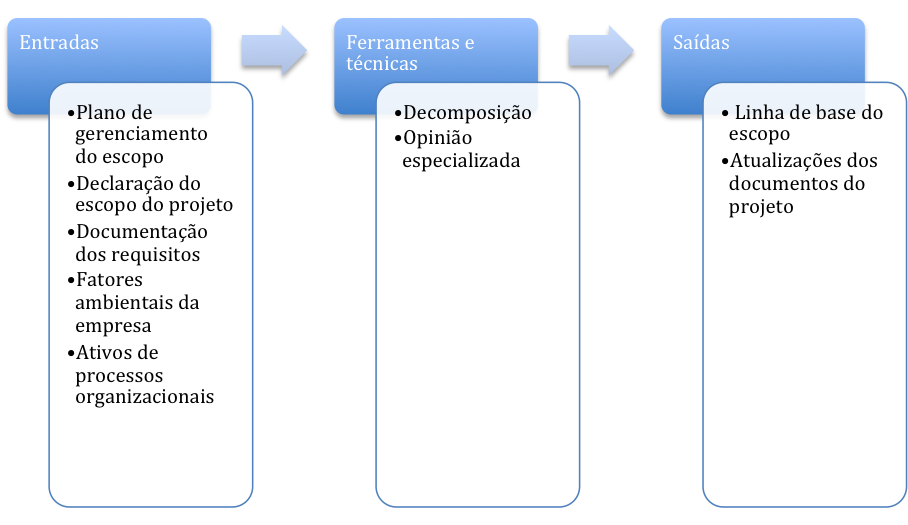
\includegraphics[scale=0.5]{Figuras/escopo_efts_EAP.png}
	\caption{Criar a EAP: entradas, ferramentas, técnicas e saídas}
	\label{fig:escopo:eap:efts}
\end{figure}

\section{Entradas}

\begin{description}
	
	\item[Plano de gerenciamento do escopo:] especifica como criar, manter e aprovar a EAP.
	
	\item[Declaração do escopo do projeto:] descreve o trabalho que será (e não será) realizado e as restrições (internas ou externas) que podem afetar a execução do projeto.
	
	\item[Documentação dos requisitos:] essencial para entender o que precisa ser produzido.
	
	\item[Fatores ambientais da empresa:] padrões específicos da indústria para a qual o projeto será realizado podem servir de referência para a criação da EAP. 
	
	\item[Ativos de processos organizacionais:] políticas, procedimentos, modelos, lições aprendidas, etc.
	
\end{description}

\section{Ferramentas e técnicas}

\begin{description}
	
	\item[Decomposição:] técnica usada para dividir e subdividir o escopo e entregas em partes menores e mais gerenciáveis.
	
	\item[Opinião especializada:] utilizada para analisar as informações necessárias para decompor as entregas em componentes menores para se criar uma EAP efetiva.
	
\end{description}

\section{Saídas}

\begin{description}
	
	\item[Linha de base do escopo:] versão aprovada da declaraçào do escopo, EAP e seu dicionário.
	
	\item[Atualizações dos documentos do projeto:] alguns documentos podem sofrer alterações no decorrer da criação da EAP, tais como a documentação de requisitos.
	
\end{description}

\chapter{Validar o escopo}

Validar o escopo é o processo de formalizar o aceite das entregas finalizadas do projeto.

O processo de validar o escopo está representado na Figura \ref{fig:escopo:validar:efts} e será descrito a seguir.

\begin{figure}[!h]
	\centering
	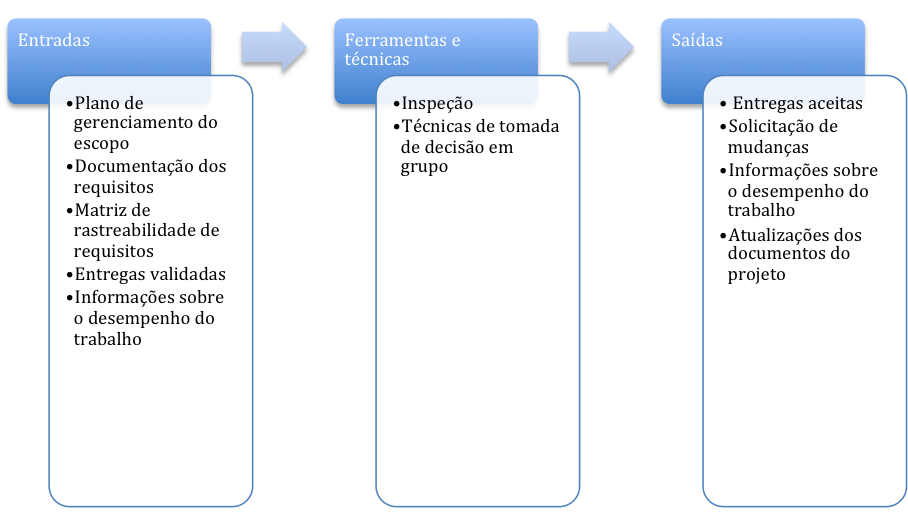
\includegraphics[scale=0.5]{Figuras/escopo_efts_verificar.png}
	\caption{Validar o escopo: entradas, ferramentas, técnicas e saídas}
	\label{fig:escopo:validar:efts}
\end{figure}

\section{Entradas}

\begin{description}
	
	\item[Plano de gerenciamento do projeto:] especifica como será obtida a aceitação formal das entregas finalzadas do projeto.
	
	\item[Documentação dos requisitos:] contém os critérios de aceitação dos requisitos.
	
	\item[Matriz de rastreabilidade dos requisitos:] liga os requisitos à sua origem e permite seu rastreamento durante todo o ciclo de vida do projeto. 
	
	\item[Entregas verificadas:] entregas finalizadas e verificadas pelo processo de controle de qualidade.
	
	\item[Informações sobre o desempenho do trabalho:] grau de conformidade dos requisitos, número de não conformidades, severidade das não conformidades ou número de ciclos de validação executados em um período de tempo.
	
\end{description}

\section{Ferramentas e técnicas}

\begin{description}
	
	\item[Inspeção:] atividades como medição, examinação e validação para determinar se o trabalho e as entregas atingem os requisitos e critérios de aceitação.
	
	\item[Técnicas de tomada de decisões em grupo:] utilizadas quando as validações são feitas em conjunto pela equipe e outras partes interessadas.
	
\end{description}

\section{Saídas}

\begin{description}
	
	\item[Entregas aceitas:] entregas que conseguem a assinatura formal de aceite pelo cliente ou patrocinador.
	
	\item[Solicitação de mudanças:] solicitações para correções de defeitos encontrados.
	
	\item[Informações sobre o desempenho do trabalho:] informações sobre o progresso do projeto.
	
	\item[Atualizações dos documentos do projeto:] o processo de validação pode alterar os documentos que dizem respeito ao escopo.
	
\end{description}


\chapter{Controlar o escopo}

Controlar o escopo é o processo de monitorar o status do escopo do projeto e do produto e gerenciar as mudanças feitas à sua linha de base.

O processo de controlar o escopo está representado na Figura \ref{fig:escopo:controlar:efts} e será descrito a seguir.

\begin{figure}[!h]
	\centering
	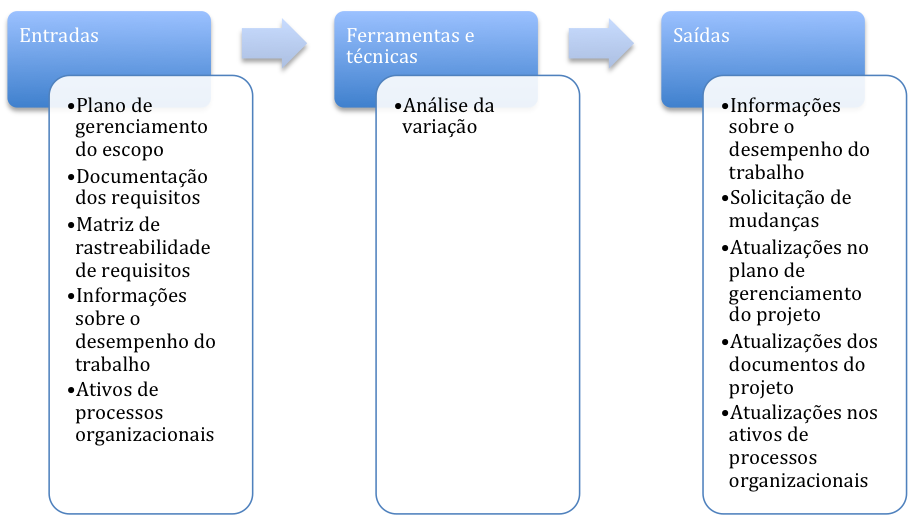
\includegraphics[scale=0.5]{Figuras/escopo_efts_controlar.png}
	\caption{Controlar o escopo: entradas, ferramentas, técnicas e saídas}
	\label{fig:escopo:controlar:efts}
\end{figure}

\section{Entradas}

\begin{description}
	
	\item[Plano de gerenciamento do projeto:] utiliza a linha de base do escopo, o plano de gerenciamento do escopo, o plano de gerenciamento de mudanças, o plano de gerenciamento da configuração e o plano de gerenciamento dos requisitos.
	
	\item[Documentação dos requisitos:] auxilia na detecção de desvios no escopo.
	
	\item[Matriz de rastreabilidade dos requisitos:] auxilia a detectar os impactos das mudanças ou desvios na linha de base do escopo sobre os objetivos do projeto. 
	
	\item[Informações sobre o desempenho do trabalho:] número de solicitações de mudança recebidas, número de solicitações aceitas e número de entregas completadas.
	
	\item[Ativos de processos organizacionais:] políticas de controle de escopo pré-definidas, modelos de monitoramento e relatórios, etc.
	
\end{description}

\section{Ferramentas e técnicas}

\begin{description}
	
	\item[Análise de variação:] técnica para determinar a causa e grau de diferença entre a linha de base e a performance real.
	
\end{description}

\section{Saídas}

\begin{description}
	
	\item[Informações sobre o desempenho do trabalho:] informações de como o projeto está progredindo comparado com sua linha de base.
	
	\item[Solicitação de mudanças:] a análise da performance do escopo pode resultar em solicitações de mudança na sua linha de base e outros componentes.
	
	\item[Atualizações dos plano de gerenciamento do projeto:] atualizações nas linhas de base do escopo e outras.
	
	\item[Atualizações dos documentos do projeto:] o processo de controle pode alterar os documentos que dizem respeito ao escopo.
	
	\item[Atualizações dos ativos de processo organizacionais:] focados principalmente nas causas das variações.
	
\end{description}